\clearpage
\section{Interim results of September 26, 2026 (UTC)}
\subsection{Accepted state at 6.2875 seconds}
This documentation snapshot, captured September 26 at 14:46 UTC
(10:46 EDT), ends at accepted step 488; the planned horizon
remains \SI{7}{s}. No future solver result is included. Only one row has been
removed: \SI{0.01984375}{mm} removed and \SI{4.74265625}{mm} still present
geometrically. The remaining thickness is not necessarily virgin material.
The mean hot-face temperature reaches \SI{1518.25}{\celsius}. The exported
nodal maximum also rounds to \SI{1518.25}{\celsius}; maximum local conversion is
\(\alpha_{\max}=1\), without implying complete conversion of the liner. The face mean and nodal maximum remain
distinct quantities.

\begin{figure}[H]\centering
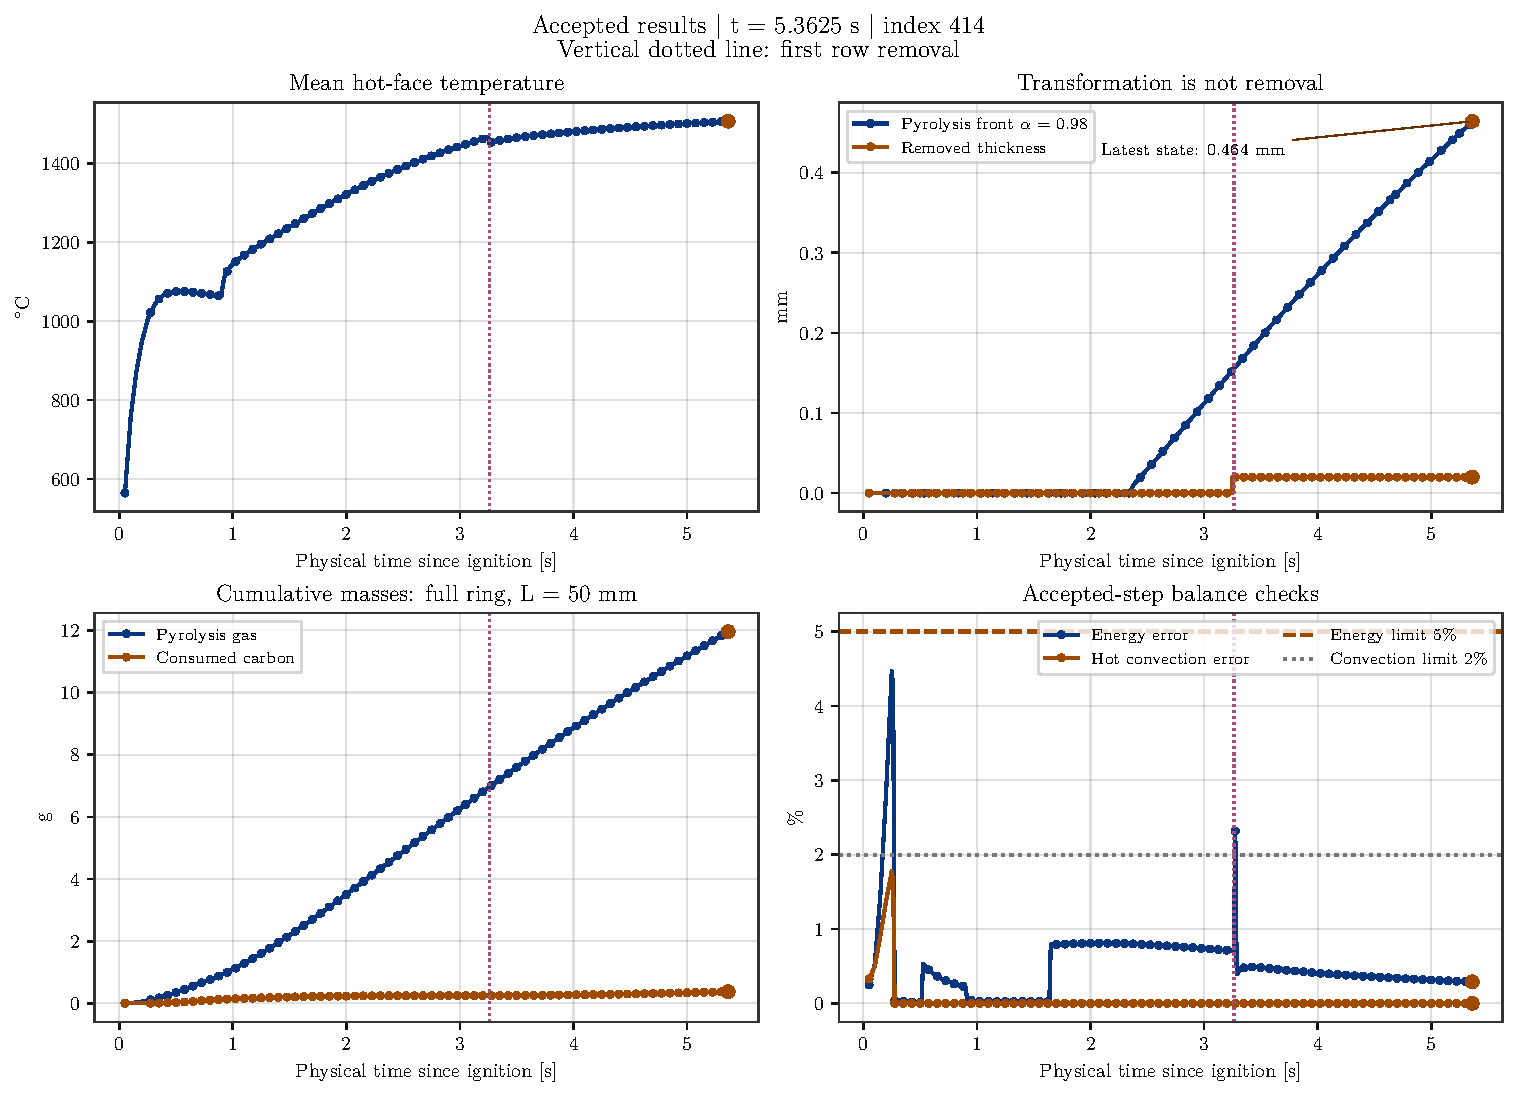
\includegraphics[width=.98\textwidth]{../analysis/newmotor_results_en.pdf}
\caption{Accepted history: mean hot-face temperature, pyrolysed depth and
geometric removal, cumulative masses, and balance errors. Masses are scaled
to a full ring of \SI{50}{mm} length. The vertical dotted line marks the
first row removal.}
\end{figure}

At the latest state, the relative energy error is 0.2406\,\% (5\,\% limit)
and the relative hot-convection error is \(5.67\times10^{-8}\) (0.02 limit).
Cumulative gas mass is \SI{13.8437}{g} and consumed-carbon mass is
\SI{0.47650}{g}, on the full-ring scale. All accepted audits are below both
limits. This validates these numerical checks, not the exploratory material
laws.

\clearpage
\subsection{Pyrolysis-front progression}
For consistency with the previous estimates, the front is defined by
\(\bar\alpha\geq0.98\), where \(\bar\alpha\) is the volume-weighted mean of
the 500 elements in a radial row. We retain the contiguous zone from the
original bore and interpolate linearly between row centres bracketing the
threshold. Already removed rows retain their last accepted conversion in
this original-bore depth measure.

\begin{figure}[H]\centering
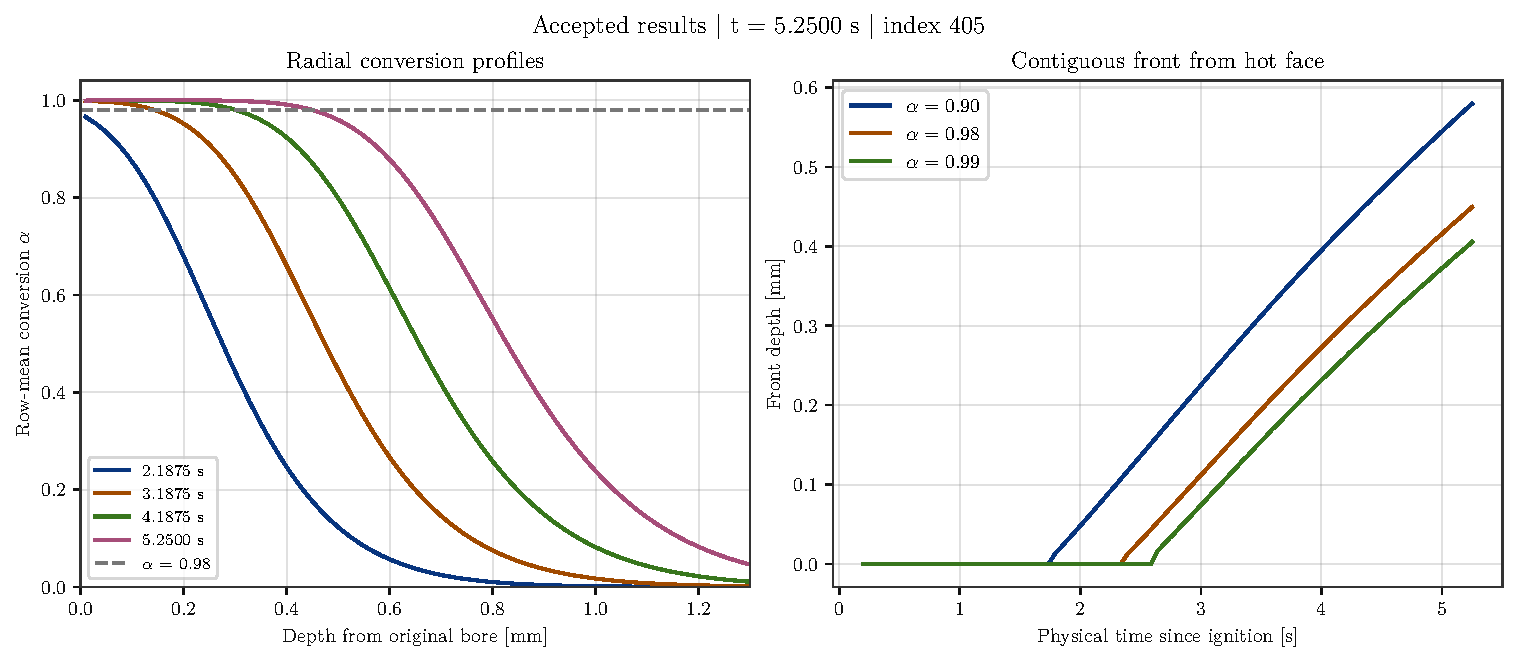
\includegraphics[width=.98\textwidth]{../analysis/newmotor_conversion_en.pdf}
\caption{Conversion profiles and depths of the 90, 98, and 99\,\% fronts.
Profiles show the first \SI{1.3}{mm} of the original \SI{4.7625}{mm} thickness.
Front histories sample every fourth checkpoint, supplemented by the latest
accepted state and the previous comparison checkpoint.}
\end{figure}

At \SI{6.2875}{s}, the 98\,\% front is at \SI{0.57986}{mm}, or 12.18\,\% of
the initial thickness. The 90 and 99\,\% fronts are at \SI{0.71616}{mm} and
\SI{0.53394}{mm}, respectively. The threshold is a post-processing definition:
it changes neither the material law nor the removal rule.
\textbf{Pyrolysed therefore means neither burned nor geometrically removed.}

\clearpage
\subsection{25, 50, and 75 percent projections}
A least-squares straight line is fitted to the 98\,\% front depth over the
latest available \SI{0.6625}{s}, using the same sampling. The current fit
uses 14 points from \SI{5.6375}{s} to \SI{6.2875}{s}. Its fitted speed is
\SI{0.12370}{mm.s^{-1}}, versus \SI{0.12822}{mm.s^{-1}} in the previous
report at \SI{5.8875}{s} (index 456).

\begin{table}[H]\centering
\caption{Physical times since ignition, not wall-clock calculation durations.}
\begin{tabular}{lrrr}\toprule
Pyrolysed initial thickness & Previous [s] & Updated [s] & Change\\\midrule
25\,\% & 11.03 & 11.22 & +1.7\,\%\\
50\,\% & 20.32 & 20.85 & +2.6\,\%\\
75\,\% & 29.60 & 30.47 & +2.9\,\%\\\bottomrule
\end{tabular}
\end{table}

\begin{figure}[H]\centering
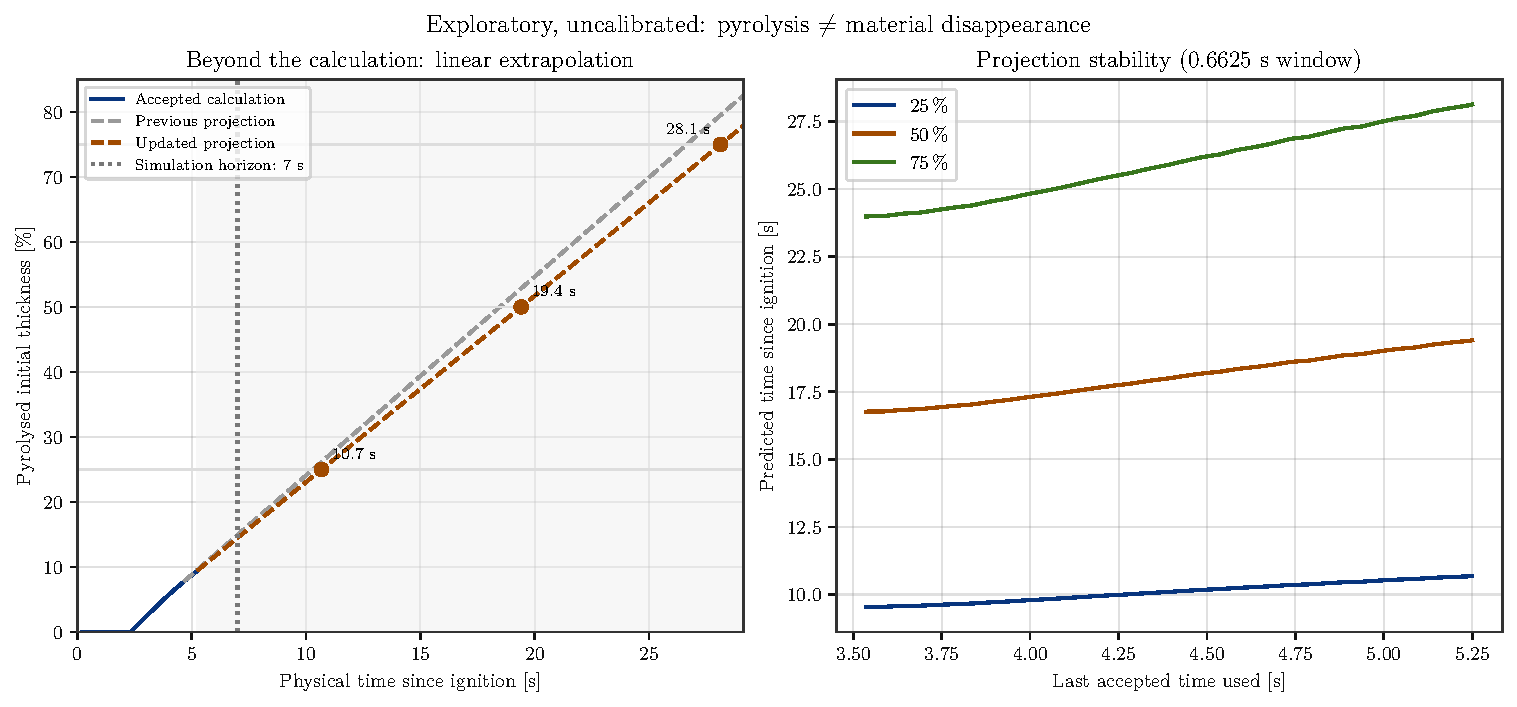
\includegraphics[width=.98\textwidth]{../analysis/newmotor_projections_en.pdf}
\caption{Left: accepted calculation in solid blue and extrapolations in
dashes; shading extends beyond available results. Right: drift in predicted
crossing times as new checkpoints enter the fitting window.}
\end{figure}

The projection at \SI{7}{s} is approximately 14.03\,\% pyrolysed. The
25/50/75\,\% estimates rise by 1.7 to 2.9\,\% since the previous report
as the front slows. This drift does not establish predictive convergence. All these
crossings lie beyond the currently authorised horizon. These are uncalibrated
linear extrapolations, with no physical confidence interval; they do not
demonstrate motor survivability. Uncertainty grows substantially at 50 and
75\,\%.

\clearpage
\subsection{Estimated completion of the 7-second calculation}
At accepted step 488, \SI{6.2875}{s}, 57 macro-steps of
\SI{0.0125}{s} remain, covering \SI{0.7125}{s} of physical time. All ten ranks
are active; step 489 at \SI{6.3}{s} has converged but is still finalising.
Its work is not counted as accepted. No new error or row removal is observed.

Throughput is calculated from accepted-audit modification timestamps over
the last 10, 20, and 30 intervals between ordinary accepted post-restart steps,
ending at step 488. Recovery of step 424 and the first acceptance interval
ending at step 425 are excluded. Neither downtime nor current-step age is
credited against remaining work. Subsequent wall-clock slowdowns remain included.
The dates below start at snapshot capture, September 26 at 10:46 EDT,
and assume constant subsequent throughput.
\begin{table}[H]\centering
\caption{Constant-throughput scenarios at snapshot capture.}
\begin{tabular}{lrrl}\toprule
Window & Minutes/step & Remaining [h] & Estimated finish (EDT)\\\midrule
10 steps & 35.86 & 34.1 & September 27, around 20:50\\
20 steps & 34.14 & 32.4 & September 27, around 19:12\\
30 steps & 40.35 & 38.3 & September 28, around 01:06\\\bottomrule
\end{tabular}
\end{table}
The last six intervals alone yield \SI{36.19}{min} per step and approximately
\SI{34.4}{h} remaining. The 30-step window includes the long step-467
finalisation interval; it is not treated here as CPU time.
\textbf{Conservative planning envelope: approximately 35 to 50 hours from
this snapshot}, or September 27 around 22:00 through September 28 around
13:00 EDT (September 28 around 02:00 through 17:00 UTC). This updates the
65-to-95-hour envelope in the step-456 report, using remaining work and
observed throughput rather than subtracting elapsed time.
It is neither a confidence interval nor a guaranteed bound. The cause of the
throughput variations is not established here; writes, exports, or row removals
may delay completion further. This estimate concerns only
completion of the \SI{7}{s} calculation, not liner disappearance or the
extrapolated 25/50/75\,\% crossings.

\subsection{Sources and reproducibility}
The \code{newmotor_v0_history.csv} history is a view of immutable JSON audits
for each accepted step: time, thicknesses, masses, surface temperature,
conversion, loads, and balances. Figures read accepted audits and conversion
checkpoints directly, never a step still being exported. The reduced snapshot
and source SHA-256 hashes are stored in
\path{docs/analysis/accepted_results_snapshot.json}. The
\code{make_results_figures.py} script rebuilds figures offline; its
\code{--capture} option reads the runtime without changing the calculation.
Text and tables in this edition are frozen at the same index 488. Audit
timestamps and all three wall-clock scenarios are preserved in this snapshot.
\clearpage
